%
% The manuscript for P1EDA. 

\documentclass[11pt,letterpaper]{article}
\usepackage{naaclhlt2015}
\usepackage{times}
\usepackage{latexsym}
\usepackage{amsmath,amssymb}
%\usepackage{microtype}
\usepackage{graphicx}
\usepackage{rotating}
\setlength\titlebox{6.5cm}    % Expanding the titlebox

\title{An extendable, multilingual textual entailment engine by
  multi-level alignments} 

\author{Author 1\\
	    XYZ Company\\
	    111 Anywhere Street\\
	    Mytown, NY 10000, USA\\
	    {\tt author1@xyz.org}
	  \And
	Author 2\\
  	ABC University\\
  	900 Main Street\\
  	Ourcity, PQ, Canada A1A 1T2\\
  {\tt author2@abc.ca}}

\date{}

\begin{document}
\maketitle
\begin{abstract}
 abstract text 
\end{abstract}

\section{Introduction}
One key challenge at the core of Natural Language Processing (NLP) is
the ability to determine which conclusions can be inferred from a
given natural language text. An engine that answers this problem,
recognition of Textual Entailment (TE), has the potential to become
the generic semantic processing engine for various NLP tasks.    

TE technology has matured over the last decade. TE modules are being
utilized in various semantic applications, and researchers can
find a range of well developed algorithms, methods and even software
suites.
It is now much easier for new users to use TE engines for their
applications. Recent developments of ``platform approach'' even permit
us to exchange various modules (such as knowledge-bases,
pre-processing pipelines) in a standardized way \cite{}.    

However, one core-problem still remains, and hinders improvements of 
existing TE solutions: extensibility of TE core algorithm
implementations. Unlike pre-processing or knowledge resources, 
extending an existing TE algorithm implementation is generally a very
difficult task. Core-algorithm parts of TE engines are normally
designed as ``black-boxes''. Thus, adding a new aspect of analysis, or
change the internal representation to a new one from an existing
engine is often very hard, if not impossible. This often forces the
next generation of TE researchers to write their own core algorithms
again from the scratch.   

In this paper, we focus and revisit this aspect of extensibility of TE
core algorithm. We propose a solution to this problem by proposing a
TE system data flow that revolves around a layer called ``multi-level
alignment'' representation that holds various heterogeneous analysis
results. Each analyzer represent their analysis as a form of alignment
between the Text (T) and Hypothesis (H). The layer works essentially
as the central representation space for the proposed TE processing
flow, and make it easier to future contributors to add their own
analysis components
%, and essentially make the core-algorithm as an
%open box, instead of a black-box. 

This paper introduces our pilot study of this architecture, and the
resulting open source multilingual TE engine implementation that works
for English, German and Italian. The implementation is a test-bed,
which utilizes only a minimal number of analyzers (aligners), coupled
with a set of basic language-independent features. The reported result
can be regarded as the baseline for this approach. Surprisingly, the
results are quite good and it already competes with best open source
engines available for each language.     

%We introduce the approach in section 2, and describe current pilot
%implementation in section 3. The section also shows multilingual
%evaluation results on the RTE-3 test-set, and on an application test
%set.  

\section{Multi-level alignment-based approach}
Alignments between Text and Hypothesis have been used as important
indicator for entailment recognitions, relatively early in the
literature. Word and phrase level monolingual aligners had been used
to find out corresponding local parts between T-H \cite{}, and also
dependency-node level alignments have shown useful for TE decisions
\cite{}.     

More generally, it is possible to map various TE approaches
conceptually fit into alignment-based approach. Ido et al. outlined
vaiours TE approaches found in the literature conceptually into a
generic alignment-based architecture that has six steps:
{\em pre-processing}, {\em enrichment}, {\em candidate alignment
  generation}, {\em alignment selection}, and {\em classification}
\cite{}.   
It is informative to compare our proposal of multi-level alignment
approach with this conceptual steps. The figure \ref{fig:1} shows the
data flow of the proposed approach. 

\begin{figure}[t!b]
  \centering
  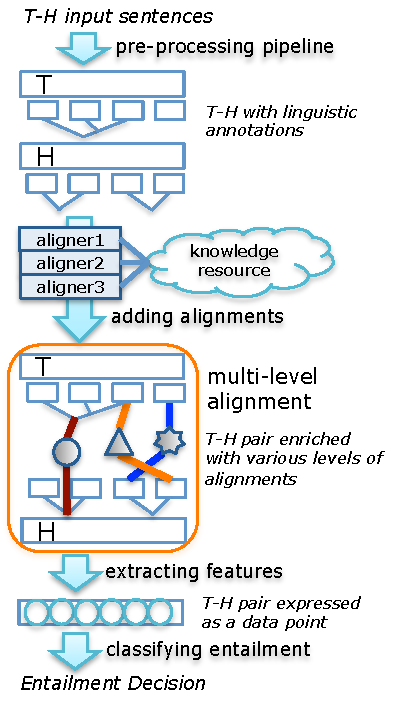
\includegraphics[width=0.8\columnwidth]{figures/figure1.pdf}
  \caption{Dataflow of the proposed approach}
  \label{fig:1}
\end{figure}

The Text (T) and Hypothesis (H) pair first get pre-processing, such as
POS tagging, lemmatizer, dependency parser and NER. Then, the 
annotated T and H pair becomes the input for various individual
aligners. Each aligner in the figure can use knowledge resources
(hence, {\em enrichment} step is abstracted within each aligner in
this setup).

Once each individual aligner adds alignments, we have a data
representation that holds all aligner outputs stored in one data
structure. This is named as ``{\em Multi-level alignments}'' in the 
figure. We envision that this representation can hold different layers
of alignments: for example, alignments that links surface level
(tokens), lemma levels, syntactic levels (e.g. dependency structures),
predicate levels, and so on. Also, analysis results normally not
treated as alignment, can be expressed here as its own alignment
expression; such as negation analysis result (e.g. this verb on T is 
negated on H), or predicate incompatibility (e.g. main verb on T
express ``possiblility'', while main verb on H express ``actuality'',
etc).   

Then the next step comes as feature extraction. With this step,
various features are extracted from the available alignments
(essentially local-analysis results reported from the aligners), and
the extracted feature vector finally represent
Finally it is classified via a general classifier trained with
training data.

One notable deviation from generic alignment-based architecture is
that, here we intentionally leaving out the step of {\em alignment 
  selection}. Alignment selection is a process where the system
finalizes alignments, by explicitly assigns a specific portion of T to
another specific position of H as the one correct alignment. Our
choice of not doing alignment selection is closely related to the fact
that we envision multi-level alignments to hold non-traditional
alignments which cannot easily mapped into one single
alignment. Getting the global view of the T-H pair is done via the
feature extraction steps. So basically, adding additional aligner
requires designing additional features. 

% 
The main (new) idea of this paper here is that making this layer of
expressed multi-level alignment structure as open as possible for
future addition of new aligner / alignments. We believe this can be
done by making this structure clearly defined, and also making the
whole algorithm (code, implementation) very easy to understand and
access. This layer is  represented with a common data type we borrowed
from \cite{}, and we added {\em alignment links} as a generic type
that can link any annotations. This enabled us to represent
multi-level alignment layer that can hold any (even future) alignment
analysis outputs.   

Naturally, this comes with a cost that each aligner (analysis)
developer need to learn how to access this common data strcuture.
We believe this is an acceptable cost, expecially when this data
structure already comes with good representation of multi-lingual,
extensible annotation data representations (see section
\ref{sec:impl} for the adopted data type). One major point of the
architecture is enabling {\em orthogonality} \cite{} between analysis
modules: adding a new (future) module (here, analyzer / aligner)
without need to know about what other modules (other aligners) are
doing. We show this is true for the proposed architecture in the next
section, with a minimal setup of aligners.    

\section{Implementation and Evaluation}
\label{sec:impl}
We report a pilot study that test the potential of the proposed
architecture. This section first describes the implementation detail,
and then shows the evaluationon of the system on RTE-3 and on an
application data-set. All the implementations with source code can
be accessed from the homepage \footnote{{URL} anonymized.}.  

\subsection{Pre-processing, knowledge components, and data representation} 
We used an open source TE development platform \cite{} as the
supporting tools for our architecture. The platform provides various  
multilingual pre-processing pipelines, and also supports a set of
knowledge resources wrapped in a standardized manner for our three
target languages (German, Italian, and English). Among the available
set of multilingual pre-processing pipelines, we have used Maltparser
with TreeTagger, for all three target languages. All knowledge
resources (such as WordNet, VerbOcean, etc) reported in this paper
are accessied via the platform. 

Another important service that is provided by the platform is the
capability of representing complex data types in a common data
representation. The platform uses UIMA CAS as the data container, and
defines various annotation types which can be extended in a coherent
manner. This naturally includes normal linguistic annotations (such as
POS, lemma, parse tree, NER...), but it also includes the ability to
add new meta data type, such as alignments. This enabled us to define
a multilingual ``multi-level alignment''  representation layer, with
minimal new data type definitions.

By utilizing those existing modules of a common platform, we were able
to concentrate on the core-algorithm implementations.   

\subsection{The minimal aligners}
We used two main aligners for this pilot study. Lexical aligner that
works on lemmas, and phrase aligner that works on consecutive tokens. 

Lexical aligner works by looking up possible connections between T-H
lemmas. The aligner add links if 

(lexical aligner works via lexical resource, add links that means this
two are related locally. all links has directions, according to the
lexical resources. Each resource become one aligner that links lemmas)

(Phrase aligner, difference, surface level (tokens).)  

(Both lexical and phrase aligner requires scan phase of T-H. We
implemented a linear time look up routine.)

Note that the two aligners are really minimal in the proposed setup,
and they are also language independent in this study. These minimal
aligners provide a test-bed baseline where additional analyzer
(aligner) developers can observe their improvements on it. 
Developing and using more sophisticated aligners for each language is
future work of this study. 

\subsection{The minimal features} 
We used four basic, language independent features in this pilot
study.

(adding proper feature according to new analyzer is
non-trivial. future work) 


\subsection{Experimental results} 
RTE3 was one of the evaluation workshop for TE \cite{}. The evaluation
data holds 800 training and 800 testing T-H pairs, and later it was
translated to both German and Italian \cite{}. As far as we know, this
is the only RTE evaluation data that is available in multiple
languages. The following table shows the evaluation result of the
pilot study, marked as {\em proposed}, compared to other open-source
TE systems that we have tested against. 

\begin{table}[t!]
\centering
\small
\begin{tabular}{l|ccc}
          &   English   &   German   &   Italian \\
\hline
{\em proposed}&   0.6700      &   0.6450    &  0.6537  \\
BIUTEE        &   0.6700      &     -       &     -    \\
TIE           &   0.652       &   0.6312    &     -    \\ 
EDITS         &   0.6362      &     -       &  0.6262  \\
RTE3 median   &   0.6100      &             &          \\

\end{tabular}
\caption{Evaluation result on RTE3 data set (accuracy).}
\label{table:rte3}
\end{table}

Each of the system is configured with their known best configurations
as reported by the developers. The pilot system supports all three
languages, while others supports one (BIUTEE, English only) or two
languages (EDITS, TIE). The pilot system performed well in all
three languages and scored the best among the tested systems.

Second task for evaluation is Entailment Graph building. It is an
application task that helps readers to explore texts in statement
levels. An entailment graph is a directed graph, where nodes
represents statements, and edges represent entailment relations
between them. Building of the graph requires a TE engine, and the TE
engine can be evaluated in this setup with F-1 measure (how effective
it was in searching for correct entailment-edges). They are texts from
customer interaction domain, and they provide large training / test
set for TE (5300 pairs for English training / testing, 1700 pairs for
Italian, etc). See \cite{} and \cite{} for more information about the
task and data.
%Previously it is reported that BIUTEE was the best available engine
%for English, and EDITS was the best for Italian \cite{}. 
Table \ref{table:egraph} shows our evaluation results.      

\begin{table}[t!]
\centering
\small
\begin{tabular}{l|ccc}
              &   English    &   Italian   &  German  \\
\hline
{\em proposed}&   0.6915     &   0.6949    &   0.7240  \\
BIUTEE        &   0.7125     &     -       &     -     \\
EDITS         &      -       &   0.6562    &     -     \\
TIE           &      -       &     -       &   0.7241  \\ 
\end{tabular}
\caption{Evaluation result on entailment graph data (f-1 measure)}
% balanced, pure-split data set. 
\label{table:egraph}
\end{table}

On this data-set, we ran two systems per each set: one is our proposed 
pilot system, and the other is the best engine reported for the data
set. The proposed engine beats EDITS in Italian data, and closely
follows German data, while BIUTEE outperforms the pilot system in
English.    

The two evaluations show that the pilot system is already competing
with the state-of-the-art open-source TE engines. The pilot system
actually outperforms in RTE3 evaluation data. The fact is even more
impressive that it is one system that works on all three languages
with minimal (language independent) aligners and features. We
interpret this result as a positive sign for the future of the
proposed architecture.     

\section{Conclusion (0.5 page)}


   %% * Results: it works! May not be as good as best alignment-based systems
   %%   BUT is extensible, robust, and multilingual
   %% * AND it is available and anyone can use it, not some research prototype (!!!

   Cite.. \cite{Katz:1987}.

%% \section*{Acknowledgments}

%% Do not number the acknowledgment section.
\bibliographystyle{naaclhlt2015}
\bibliography{sem2015_short}

\end{document}
